For at danne overblik over software-udviklingen inden det egentlige design laves bruges N+1 modellen.
Denne beskriver fire faser som tager hånd om de overordnede ting inden for software, alt sammen med use-cases som den røde tråd.
De fire fase er:
\begin{enumerate}
	\item Logical View
	\item Deployment View
	\item Implementation View
	\item Data View
\end{enumerate}

Ud over disse punkter tænkes der også en overordnet fejl-håndtering ind i projektet samt skitser for den grafiske brugerflade. Disse punkter er beskrevet i detaljer her efter.

\subsection{Logical View (JSA)}
%% SW arkitektur: Logical View

Logical View skal danne et overblik over hvilke softwarepakker der befinder sig på platforme. Blokkene inde i de respektive pakker kan sammen med domænemodellen, hjælpe med at give et overblik over hvilke klasser og kernemoduler der skal bruges.

\begin{figure}[htbp] \centering
{\includegraphics[scale=0.7]{filer/systemarkitektur/logical_view_devkit}}
\caption{Logical view for Devkit8000 illustrerer hvilke softwarepakker der befinder sig på Masteren }
\label{fig:Logical View Devkit8000}
\end{figure}

Figur \ref{fig:Logical View Devkit8000} illustrerer hvilke softwarepakker der ligger på Masteren. I bunden er \textit{Device drivers}-pakken som håndterer SPI kommunikationen imellem Master og Enhed. I midten ligger \textit{Hardware API}-pakken som håndterer protokol-vedtægter ifm. kommunikationen. \textit{Application}-pakken tager sig af alt UI samt log og fejlhåndtering.

\clearpage

\newenvironment{figure1}[1][]{\begin{figure}[#1]\vspace{3.0cm}}{\vspace{1.0cm}\end{figure}}
\begin{figure1}[htbp] \centering
{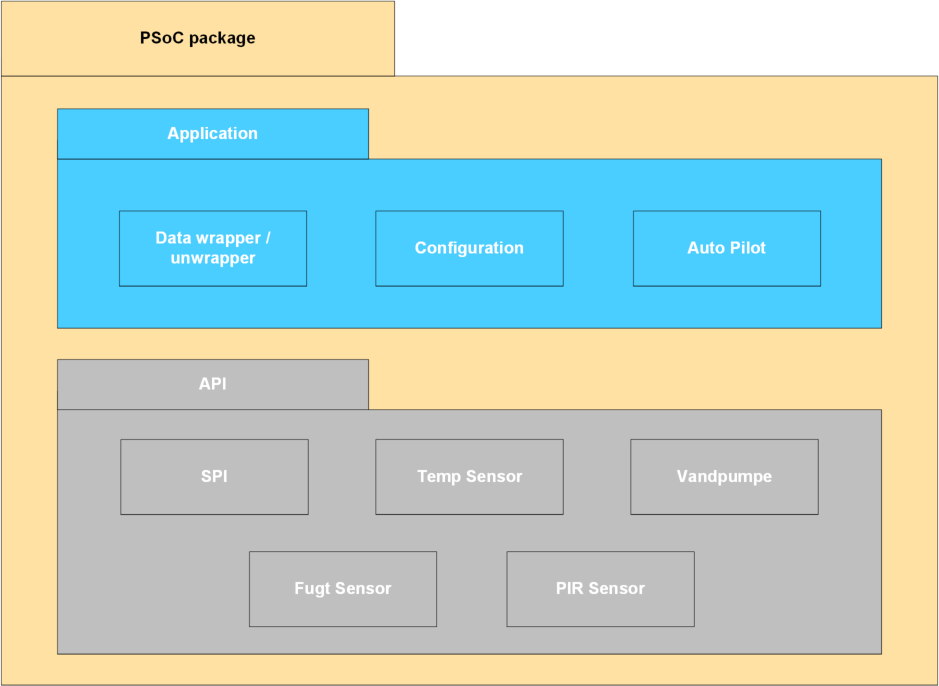
\includegraphics[scale=0.7]{filer/systemarkitektur/logical_view_psoc}}
\caption{Logical view for PSoC illustrer hvilke software pakker der befinder sig på enhederne}
\label{fig:Logical View PSoC}
\end{figure1}

Figur \ref{fig:Logical View PSoC} illustrerer hvilke softwarepakker der ligger på Enhederne. \textit{API}-pakken består af den software som håndterer hardwaren, dvs. den tager imod input og får formateret det til noget brugbart for \textit{Application}-pakken. \textit{Application}-pakken håndterer den indsamlede data som den får fra sensorene igennem \textit{API}-pakken. Denne data sammensættes iht. protokollen og sendes til API pakken som får det sendt til Devkit8000. Pakken skal også håndterer data fra Devkit8000 til at konfigurerer de parametre der styrer automatiseringen af vandingen.



\subsection{Deployment View ()}
%% SW arkitektur: Deployment View

Deployment view skal illustrere hvor hvilke lag af software ligger på vores platforme. Devkit8000 kører linux og har derfor flere software lag end PSoC'en.
 
\vspace{15 mm}

\begin{figure}[htbp] \centering
{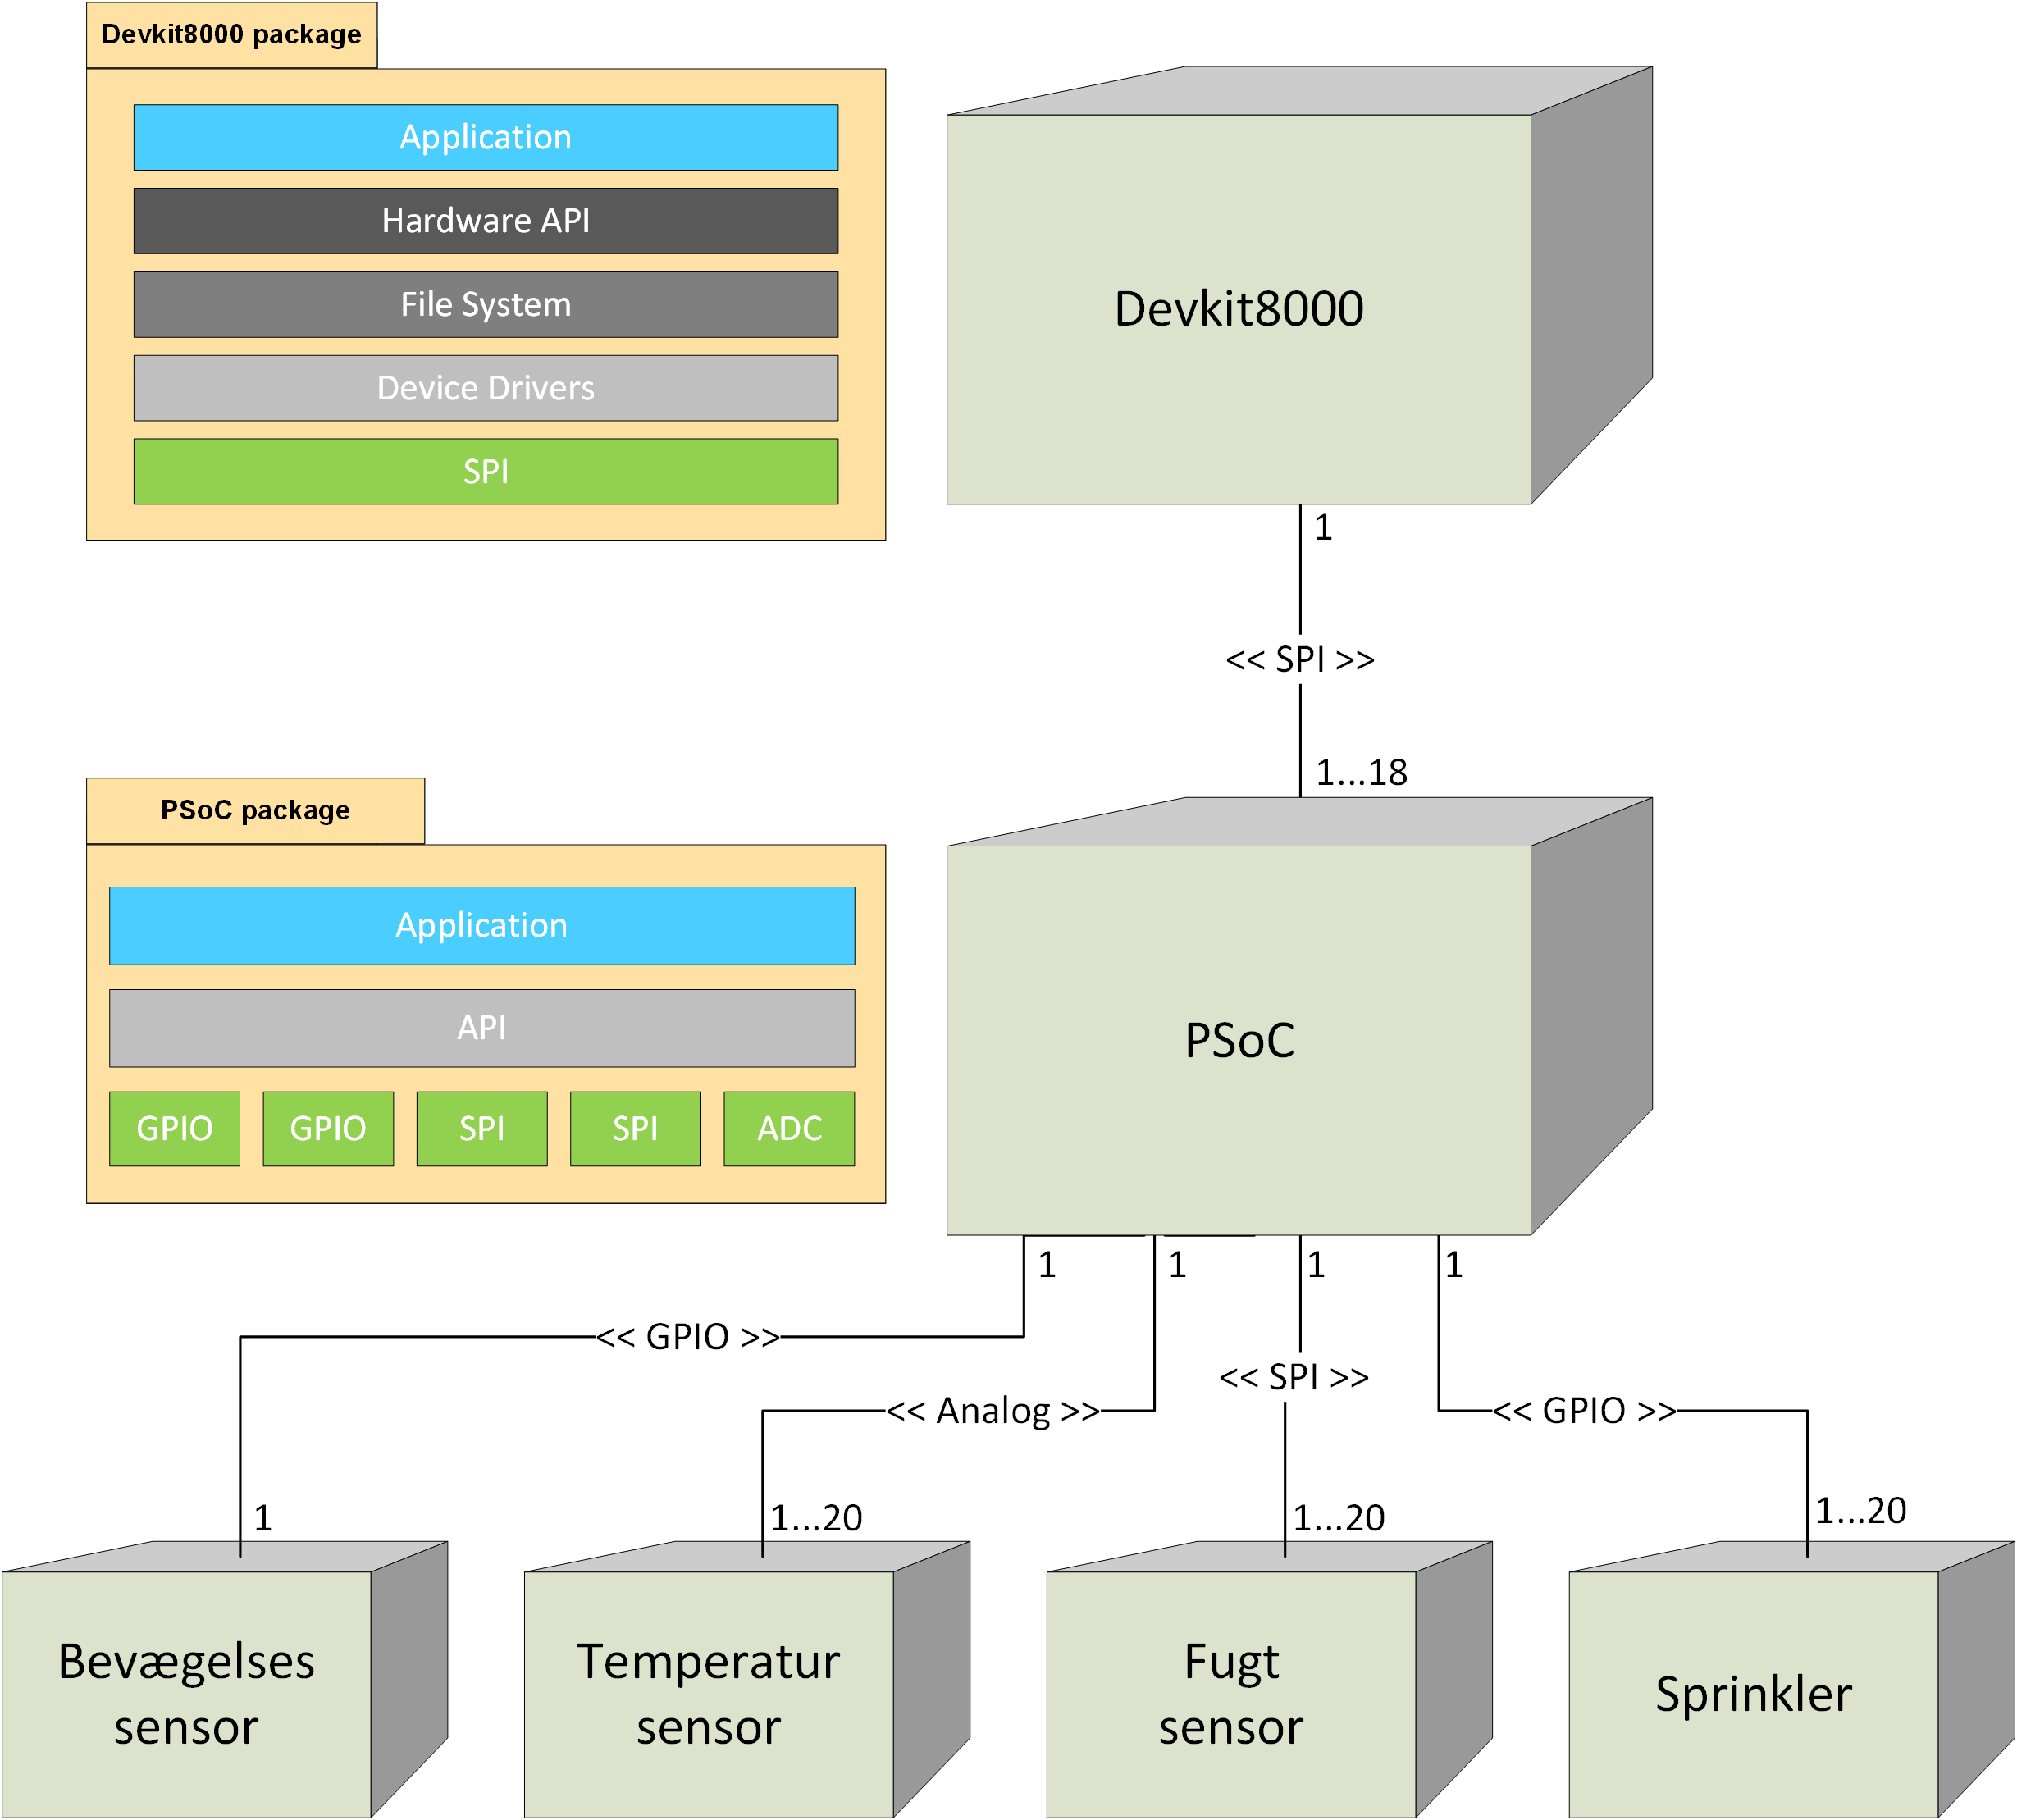
\includegraphics[scale=0.7]{filer/systemarkitektur/Deployment_model}}
\caption{Deployment model illustrere de forskellige software og hardware(grønne) lag}
\label{fig:Deployment Model}
\end{figure}

\vspace{5 mm}

\subsubsection{Devkit8000}
\textit{Applications} laget består af alt den software som har med brugeren at gøre, dvs. UI og tilhørende controllers. Applicationslaget tager imod input fra brugeren og reagere på det enten ved at kalde nogle af sine egne controllers eller sende kommandoer til hardware APIen. Laget skal desuden få data fra nedenstående lag til at fremstå overskueligt over for brugeren.

\clearpage

\textit{Hardware API} laget består af almindelige klasser som gør brug af file systemets kommandoer som f.eks open og close.

\textit{File System}

\textit{Device Driver} laget består af den software som håndtere alt hardware input og output. Hardware proxys inklusiv.

\textit{HW connection (grønne bokse)} laget viser hvilke hardware in/out der er til devkittet

\subsubsection{PSoC}

\textit{Applications} laget håndtere den indsamlede data som den får fra sensorene igennem API'en. Denne data sammensættes ifølge protokollen og sendes til API'en som får det sendt til devkittet. Laget skal også håndtere data fra devkittet til at konfigurere de parametre der styre automatiseringen af vandingen som applications laget også håndtere.

\textit{API} laget består af den software som håndtere hardwaren. dvs den tager imod input og får formateret det til noget læseligt til applications laget. Derudover står den for at få sendt de informationer applicationslaget ber om på en effektiv og sikker måde.

\textit{HW connection (grønne bokse)} laget viser hvilke hardware in/out der er til PSoC'en

\subsection{Implementation View ()}
%% SW arkitektur: Implementation View

Inden programmerne designes, fastlægges en struktur for kildekoden. På den måde er det nemmere for flere programmører at arbejde med delene i programmet samtidigt.

Strukturen skal være som vist i figur \ref{fig:implementationview}. Under mappen ''Kildekode'' skal hver klasse have en mappe med dertil hørende filer. Ligeledes med ''Testprogrammer'' mappen, som indholder testprogrammer som verificerer funktionaliteten af de enkelte moduler.
Mappen ''Kompilerede programmer'' er til de endelige programmer.

\begin{figure}[htbp] \centering
{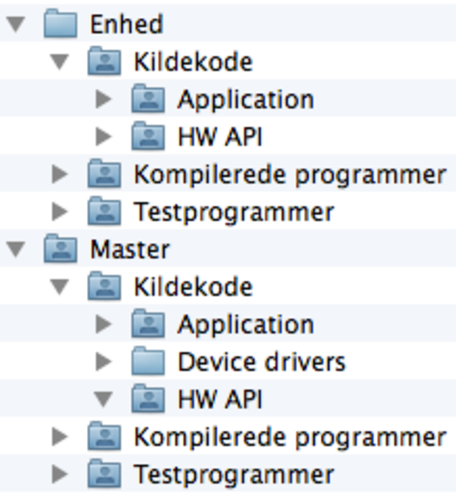
\includegraphics[scale=0.7]{filer/pics/SW-Implementation-View}}
\caption{Mappestruktur for software-kilder}
\label{fig:implementationview}
\end{figure}

\subsection{Data View (BS)}
%% SW arkitektur: Data View

I forbindelse med EasyWater8000s log skal der gemmes data på en nem og håndterbar måde. Det skal være muligt at gemme følgende data:

\begin{enumerate}
	\item Tidsstempel
	\item Temperatur
	\item Fugtighed
	\item Bevægelse
	\item Vanding
\end{enumerate}

Ydermere skal disse informationer gemmes for hver Enhed. Så hvis der er 18 huller med i alt 18 Enheder, skal ovenstående gemmes for alle 18 enheder.

Når informationen skal præsenteres for brugeren skal det ske i en tabel som vist på figur \ref{fig:GUI-log-alle} i afsnit \ref{subsec:GUI}, data for en enkelt enhed som på figur \ref{fig:GUI-log-enhed} i afsnit \ref{subsec:GUI} eller på en graf så man kan se ændringer over tid som vist på figur \ref{fig:log-graf}.

\begin{figure}[htbp] \centering
{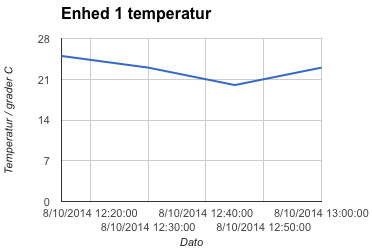
\includegraphics[scale=0.5]{filer/pics/SW-Log-graf}}
\caption{Graf for temperatur for én Enhed}
\label{fig:log-graf}
\end{figure}

Tabellen skal have en fane for hver opkoblet Enhed. Her kan man se informationer fra hver enkelt Enhed. Det bør også være muligt at se alle enheders informationer samtidigt.

Dataen struktureres i semikolon-separerede filer (\verb+.csv+) på Master. Hver Enhed har en fil hvor alle data er samlet med udgangspunkt i strukturen vist i liste \ref{list:log-csv-struktur}.

\begin{lstlisting}[caption=Semikolon-separeret datafil til log af enheder, label={list:log-csv-struktur}]
<enheds-nr>;
<KP-nr>; <dato>; <temperatur>; <fugtighed>; <bevaeglse>; <vanding>;
<KP-nr>; <dato>; <temperatur>; <fugtighed>; <bevaeglse>; <vanding>;
...
<KP-nr>; <dato>; <temperatur>; <fugtighed>; <bevaeglse>; <vanding>;
\end{lstlisting}

Dette resulterer i en filstruktur som vist på liste \ref{list:log-fil-struktur} hvis der er koblet 18 Enheder op på Master.

\begin{lstlisting}[caption=Filstruktur for logfiler på Master, label={list:log-fil-struktur}]
<log>/
  <enheds-nr1>.csv
  <enheds-nr2>.csv
  ...
  <enheds-nr17>.csv
  <enheds-nr18>.csv
\end{lstlisting}

Hyppigheden for målingerne og logningen er beskrevet i de ikke-funktionelle krav, \ref{header:ikke-funk}.


\subsection{Fejl-håndtering (JC)}
%% SW arkitektur: Fejlhåndtering

Systemet kan håndterer fejl og disse vil blive gemt i en fejllog som bliver gemt på Master. 

Fejlhåndteringen bliver klaret af en klasse på Devkit8000 som håndterer at skrive det rigtige fejl ud i en \verb+.txt+-fil. Klassen vil blive kaldt med en fejlkode hver gang fejl opstår. Klassen forstår så at skrive den rigtige fejl ind i txt filen ud fra den pågældende fejlkode den har modtaget som attribut. 

Alle funktioner vil returnere et negativt heltal som repræsenterer en fejlkoden som klassen kan tolke på.

\begin{figure}[htbp] \centering
{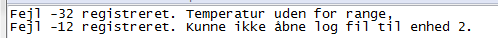
\includegraphics[scale=0.7]{filer/pics/Errortxt}}
\caption{udsnit af Error log}
\label{fig:ErrorLog}
\end{figure}

Billedet på figur \ref{fig:ErrorLog} viser hvordan 2 fejl i error-loggen kunne se ud.

\subsection{Grafiske brugerflade-skitser (BS)}
\label{subsec:GUI}
%% SW arkitektur: GUI skitser

Inden det endelige GUI udvikles laves nogle skitser som udviklingen læner sig op af. Ud fra UC beskrivelserne findes de skærmbilleder som skal vises på Master og skitseres.

Her følger korte beskrivelser af hver skitse samt skitsen selv.

\subsubsection{Startmenu}
Figur \ref{fig:GUI-Startmenu} er den første menu brugeren kommer til. Her er valgmulighederne præsenteret for brugeren.

\begin{figure}[htbp] \centering
{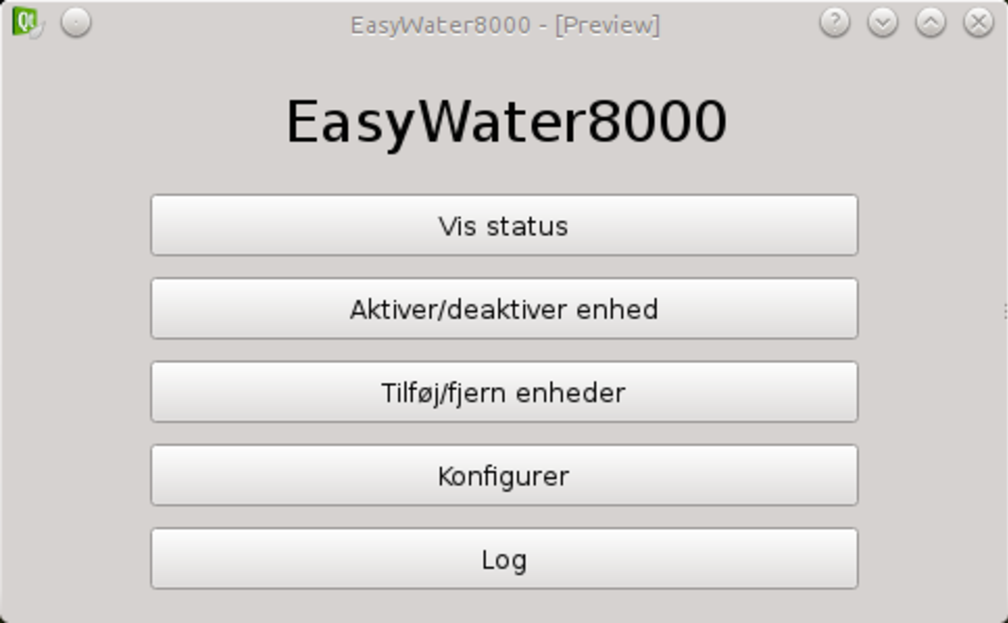
\includegraphics[scale=0.5]{filer/pics/GUI/Start-menu}}
\caption{Skitse af startmenu på GUI}
\label{fig:GUI-Startmenu}
\end{figure}

\subsubsection{Vis Status}
På figur \ref{fig:GUI-aktuel-status} vises den aktuelle status af systemets enheder. Den øverste række tal er tilkoblede Enheder. Den anden række tal er komponentpakker tilkoblet den enkelte enhed.

\begin{figure}[htbp] \centering
{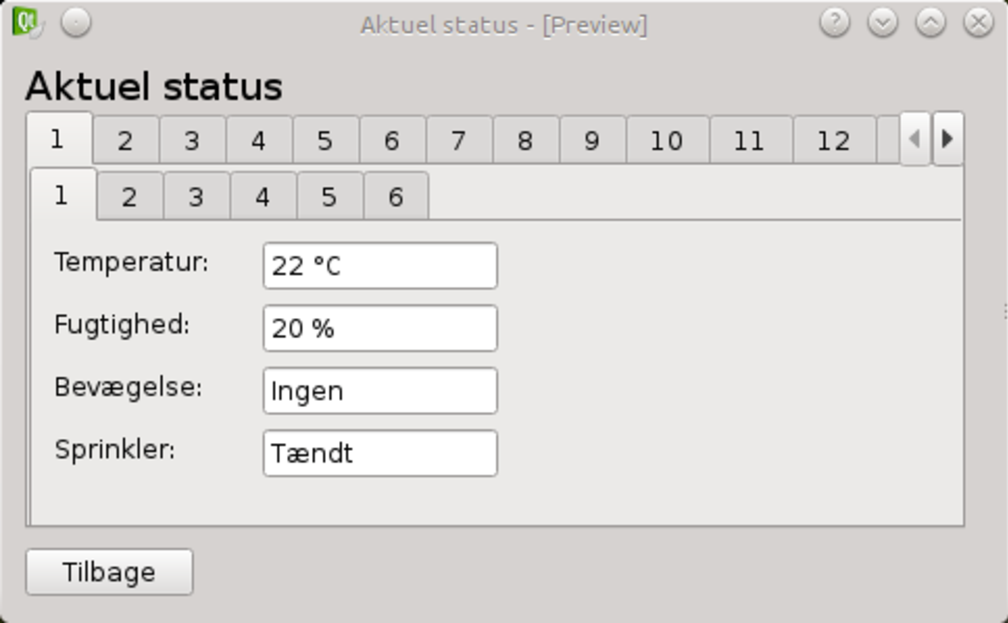
\includegraphics[scale=0.5]{filer/pics/GUI/Aktuel-status}}
\caption{Skitse af ''Vis status'' på GUI}
\label{fig:GUI-aktuel-status}
\end{figure}

\subsubsection{Aktiver og deaktiver enhed}
Skitsen på figur \ref{fig:GUI-aktiver-deaktiver} viser brugerens mulighed for at aktivere og deaktivere enkelte enheder i systemet.

\begin{figure}[htbp] \centering
{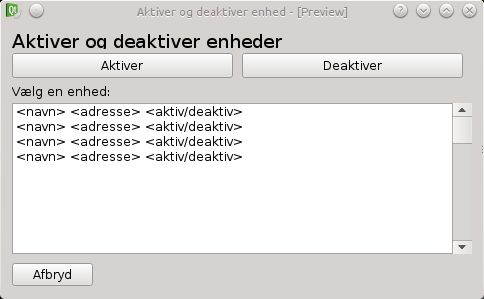
\includegraphics[scale=0.5]{filer/pics/GUI/Aktiver-deaktiver-enheder}}
\caption{Skitse af ''Aktiver og deaktiver enhed'' på GUI}
\label{fig:GUI-aktiver-deaktiver}
\end{figure}

\subsubsection{Tilføj/fjern enheder}
De præsenterede muligheder i forbindelse med at fjerne og tilføje enheder til systemet er vist på figur \ref{fig:GUI-tilfoj-fjern}.

\begin{figure}[htbp] \centering
{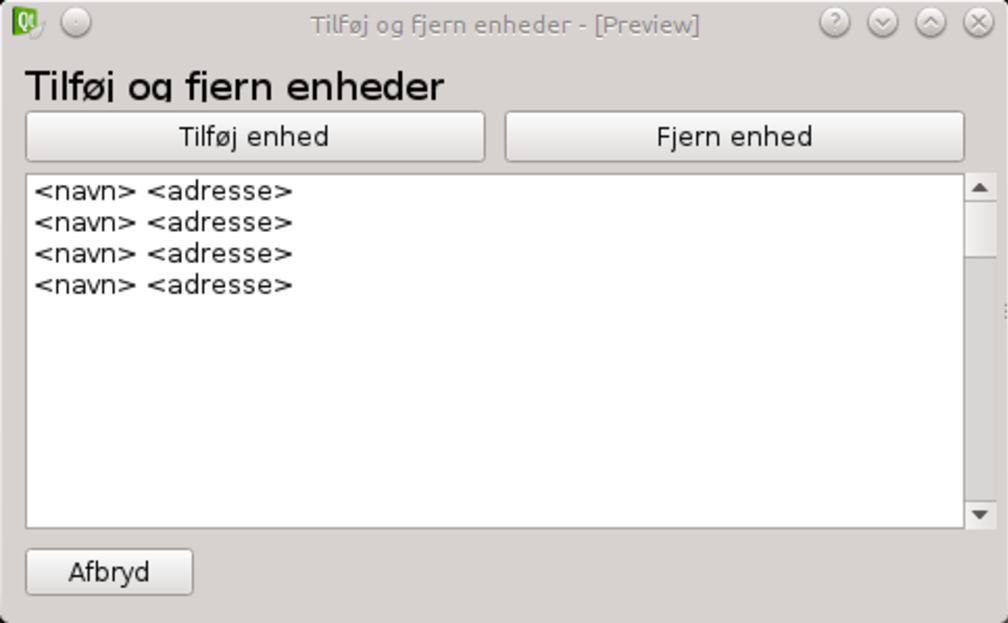
\includegraphics[scale=0.5]{filer/pics/GUI/Tilfoj-fjern-enheder}}
\caption{Skitse af ''Tilføj/fjern enheder'' på GUI}
\label{fig:GUI-tilfoj-fjern}
\end{figure}

\subsubsection{Konfigurer}
Når brugeren skal konfigurerer en enhed bruges skitsen på figur \ref{fig:GUI-konfigurer}. Her vælger brugeren hvilken enhed der skal konfigureres.

\begin{figure}[htbp] \centering
{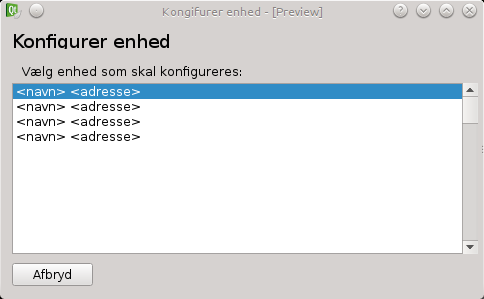
\includegraphics[scale=0.5]{filer/pics/GUI/Konfigurer-enhed}}
\caption{Skitse af ''Konfigurer'' på GUI}
\label{fig:GUI-konfigurer}
\end{figure}

\subsubsection{Indstil parametre}
Når brugeren har valgt en enhed som skal konfigureres vises skærmen på figur \ref{fig:GUI-indstil-parametre}. Her kan brugeren indtaste parametrene for enheden.

\begin{figure}[htbp] \centering
{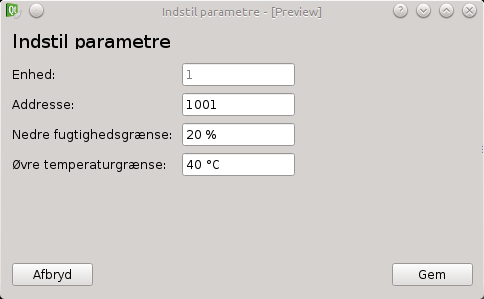
\includegraphics[scale=0.5]{filer/pics/GUI/Indstil-parametre}}
\caption{Skitse af ''Indstil parametre'' på GUI}
\label{fig:GUI-indstil-parametre}
\end{figure}

\subsubsection{Log}
Loggen præsenterer de indsamlede data fra alle enhederne. Det er muligt at se alle data på en gang, som vist på figur \ref{fig:GUI-log-alle}, hvor den øverste fanerække er numre på opsatte enheder i systemet, eller man kan vælge de enkelte enheder og se deres forskellige komponentpakker, som vist på figur \ref{fig:GUI-log-enhed}, hvor den anden fanerække er komponentpakker koblet op på systemet.

\begin{figure}[htbp] \centering
{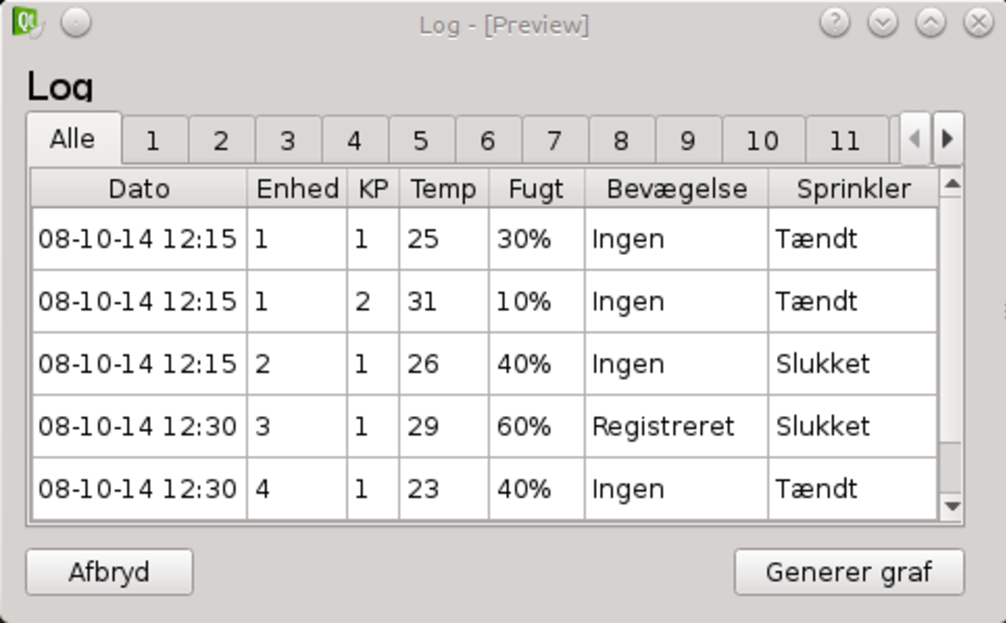
\includegraphics[scale=0.5]{filer/pics/GUI/Log-alle}}
\caption{Skitse af ''Log'' for alle enheder på GUI}
\label{fig:GUI-log-alle}
\end{figure}

\begin{figure}[htbp] \centering
{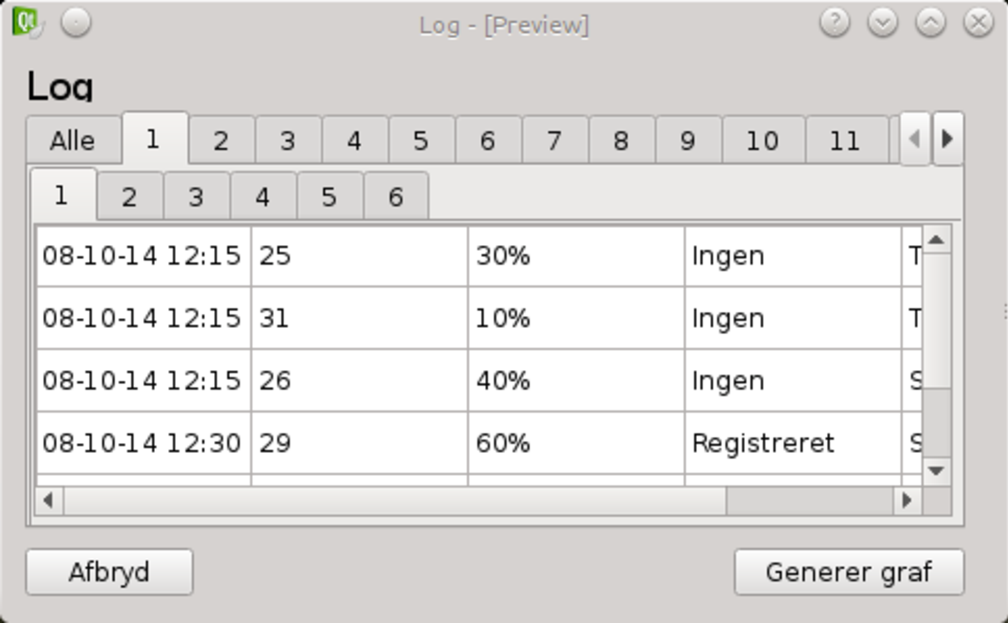
\includegraphics[scale=0.5]{filer/pics/GUI/Log-enhed}}
\caption{Skitse af ''Log'' for enkelt enhed på GUI}
\label{fig:GUI-log-enhed}
\end{figure}



